\documentclass[a4paper,11pt]{article}
\usepackage[T1]{fontenc}                  % Output font (default)
\usepackage[utf8]{inputenc}               % Font (default)
\usepackage{lmodern}                      % Latin modern (default)
\usepackage{setspace}                     % Line spacing
\usepackage{sectsty}                      % Typesetting section headings
\usepackage[protrusion=true,expansion=true]{microtype} % Pretty lay-out
\usepackage{booktabs}                     % Tables
\usepackage{graphicx}                     % Graphics
\usepackage{amsmath}                      % Math type-set
\usepackage{rotating}                     % Tables in landscape
\usepackage{latexsym}                     % Fixing table column width
\usepackage{bm,array}                     % Fixing table column width
\usepackage[tableposition=top,labelfont=bf]{caption}   % Table caption at top with bold font
\usepackage{pbox}
\usepackage{hyperref}                     % Including url's
\usepackage{subcaption}                   % Package for subcaptions
\usepackage{natbib}                       % References & bibliography
\usepackage{textcomp} 
\usepackage{pbox}
\usepackage[margin=3cm]{geometry}
\usepackage{authblk,etoolbox}             % Adjusting title page
\usepackage{abstract}

%% Adjust abstract
\renewcommand{\absnamepos}{flushleft}
\setlength{\absleftindent}{0pt}
\setlength{\absrightindent}{0pt}


%%%% Redefine title page %%%%
\makeatletter
% Patch \maketitle so that it doesn't center
\patchcmd{\@maketitle}{center}{flushleft}{}{}
\patchcmd{\@maketitle}{center}{flushleft}{}{}

% Patch the patch by authblk so that the author block is flush left
\def\maketitle{{%
  \renewenvironment{tabular}[2][]
    {\begin{flushleft}}
    {\end{flushleft}}
  \AB@maketitle}}
\makeatother

% A couple of other settings
\renewcommand\Authands{ and }
\renewcommand\Authfont{\normalfont\normalsize}
\renewcommand\Affilfont{\normalfont\normalsize}

%% Other settings
\DeclareUnicodeCharacter{00A0}{ }
\graphicspath{ {/home/swl/Dropbox/Sandbox/granborough/repBC2010} }
\hypersetup{colorlinks=true, linkcolor=blue, citecolor=blue, urlcolor=blue}
%======================================
% Title
%======================================
\title{Commodity prices, growth, and civil war revisited\thanks{Many thanks to Brückner \& Ciccone for providing their data and code as well as answering questions.}}
\author{Stijn van Weezel \\
          Department of Economics\\
          Royal Holloway College, University of London \\
          pwte054@rhul.ac.uk}
\date{}
\begin{document}
%======================================
\maketitle
\noindent
%======================================
% ABSTRACT
%======================================
\begin{abstract}
\noindent
Brückner and Ciccone (2010) find that there is a higher probability of the outbreak of civil war in Sub-Sahara Africa following downturns in the international commodity prices of the countries' main traded commodities. 
I use R to replicate their results which yields identical estimates but slight discrepancies in the standard errors due to a small sample adjustment, although this doesn't affect the level of statistical significance.
Re-estimating the model using the latest data for 1981-2013 I am unable to find a strong link between commodity price shocks and civil war but do find that economic growth in OECD export countries negatively affects civil war onset. 
\end{abstract}
\textbf{Keywords:} Replication, Conflict, Commodity prices, Africa
%**************************************
%%%% Introduction %%%%
% INTRODUCTION
%**************************************
\section{Introduction}
In a widely cited study, \citet{Bruckner2010} $-$ referred to as B\&C henceforth $-$ examine the link between economic performance and conflict focussing on the effect of international commodity prices on the outbreak of civil war. 
Using data for 39 countries in Sub-Sahara Africa they find that there is a higher probability of civil war onset following downturns in the international prices of the countries' main export commodities.\footnote{Civil wars are here defined as a contested incompatibility that concerns government and/or
territory where the use of armed force between two parties, of which at least one is the
government of a state, results in at least 1,000 battle-related deaths in a year \citep{Gleditsch2002}.} 
This relation holds across a number of different model specifications and estimations methods. 
Their results also show that the outbreak of civil war is more likely following recessions in the main OECD export destinations.
Here I present a replication and reanalysis of their work.\footnote{Please see \citet{Clemens2015} for a proposed taxonomy the definition of replication.} 
The replication focuses on reproducing their results in R to see how these compare with the original estimates which were obtained using STATA. 
For the reanalysis I update the data to include the most recent data on civil war and international commodity prices, and extend the sample period to 1981-2013 to see whether their results generalise.\footnote{Their main results were based on the years between 1981-2006. Note that the work by \citet{Bazzi2014} also revisited the B\&C study updating the data till 2007.} 
%**************************************
%%%% Replication results %%%%
%**************************************
\section{Replication results}
% Intro
The replication focuses on the main results of the B\&C study as reported in tables 2 through 6 in their article. 
For their study, the estimates were obtained estimating the model in STATA. 
Using the original code and dataset in STATA, I am able to perfectly replicate their results.\footnote{I used STATA 12.1.} 
I estimate the models in R, using the original data, in order to compare the results. 
In general I find that R produces identical estimates, at the reported number of decimals, and that in most cases the estimates have the same level of statistical significance.\footnote{Replication results can be found in the appendix.} 
There are some minor discrepancies though, for instance none of the reported $t$-values can be replicated in R.
These discrepancies are due to the differences in the calculation of the robust clustered standard errors.
In R, the heteroskedasticity-consistent estimation of the covariance matrix is done using a small sample adjustment, similar to the one used in the \textit{reg} function in STATA, but which is absent in the default of the \textit{ivreg2} function in STATA which was used to obtain the original results.\footnote{Although the authors do not elaborate on this, one reason for not using the default small sample adjustment is that the statistical theory for hypothesis testing assumes that the residuals are homoskedastic and normally distributed as explained by \citet{Ciccone2011}. These assumptions are likely violated using LPMs. \citet{Bazzi2014} found that the results by B\&C are sensitive to the use of \textit{ivreg2} without making the usual small sample adjustment (see section D.2 and table 11 in their online \href{https://www.aeaweb.org/aej/mac/app/0604/2013-0226_app.pdf}{appendix}).}
Estimating the model using the standard \textit{reg} command, with robust standard errors clustered at the country level, I get results identical to those in R for the LMPs.
Similarly, estimating the model in STATA using \textit{ivreg2} with the \textit{small} sample adjustment also produces identical results to both the \textit{reg} and R estimation results.\\
% Failure to replicate
In most cases this adjustment didn't influence the level of statistical significance of the coefficients. 
However, there was one exception: the model estimated using rare events logit \citep{King2001}, in their table 3 column 5, ceases to be statistically significant.\footnote{The \textit{p}-value was 0.10 in the original result, 0.13 in the replication in R.}\\
I only failed to replicate one result, which was the logit estimation reported in table 3 column 7. 
This model includes country and year fixed effects as well as a country-specific time trend. 
The estimated coefficient is about 16\% larger than the reported estimate.\footnote{Additionally, R gives a warning message stating that the algorithm did not converge and fitted probabilities numerically 0 or 1 occurred. This is likely the result of overfitting the model as there is little variation in the outcome variable: only 2.8\% of the observations is non-zero.} 
%**************************************
%%%% Reanalysis %%%%
%**************************************
\section{Reanalysis}
% Intro on expansion
The economic performance of African countries has steadily improved in the past decade, and as a result they might have become less reliant on the primary sector. 
Additionally, we also see that the incidence of civil war in Africa is at a relatively low level, especially compared to the high water mark of the 1980's. 
Given the trends in both economic performance and civil war, it would be interesting to check whether the results by B\&C generalise expanding the period to 1981-2013.\\\\
% Data description
I update the data to cover the years 1981-2013, using the same data sources and methodology for constructing the country-specific commodity price index and coding the war onset indicator, and re-estimate the model.\footnote{The country-specific commodity price index is constructed using the data on commodity exports provided in their table A1. Data on international commodity prices is taken from the \href{http://www.imf.org/external/np/res/commod/External_Data.xls}{IMF} which was also the primary data source for B\&C. Since this data source does not have information on international prices for gold, phosphates, and tobacco, which are included in the B\&C price index, I use the \href{http://data.worldbank.org/data-catalog/commodity-price-data}{Global Economic Monitor Commodities} to supplement. Data for real GDP growth, to measure income, is taken from the World Development Indicators (WDI) which is also what B\&C use for the later years in their sample period. WDI data is preferred over data from the Penn World Tables (PWT) due to recent concerns with high frequency PWT data \citep{Johnson2009}. For the data on civil war I used version \href{http://www.pcr.uu.se/research/ucdp/datasets/ucdp_prio_armed_conflict_dataset/}{4-2014a} of the UCDP/PRIO Armed Conflict Dataset. The IMF \href{http://elibrary-data.imf.org/QueryBuilder.aspx?key=19784661&s=322}{Direction of Trade Statistics} were used to update the variable on export-weighted OECD growth as the data source mentioned in the article is no longer available.}
% On conflict data
From the 1980's onward, civil war in Africa has been declining and since 2006 there has been a slight decrease in the rate of civil war onsets between 2007-2013 compared to 1981-2006 (see figure~\ref{fig:conflict_trends}). 
Nonetheless, the rates are still comparable: between 1981-2006 on average one civil war started each year, while for 2007-2013 we see on average one outbreak each year and a half.\footnote{According to the latest data, between 1981-2006 there were 27 civil war outbreaks compared to 5 between 2007-2013.}
Besides general trends, another issue with armed conflict data is that it is revised from time to time.\footnote{See table~\ref{table:war} for an overview of the changes in civil war onset-years per country.} 
Therefore I first check if the original results can be replicated using the updated data on conflict. 
I focus on the model given in their table 2 column 5, which regresses the onset of civil war on the commodity price growth rate between $t$ and $t-3$ including country and year fixed effects and a country-specific time trend (i.e. the reduced-form model).\\\\
%**************************************
%%%% Figure: Coefficients %%%%
%**************************************
\begin{figure}[!h]\centering
    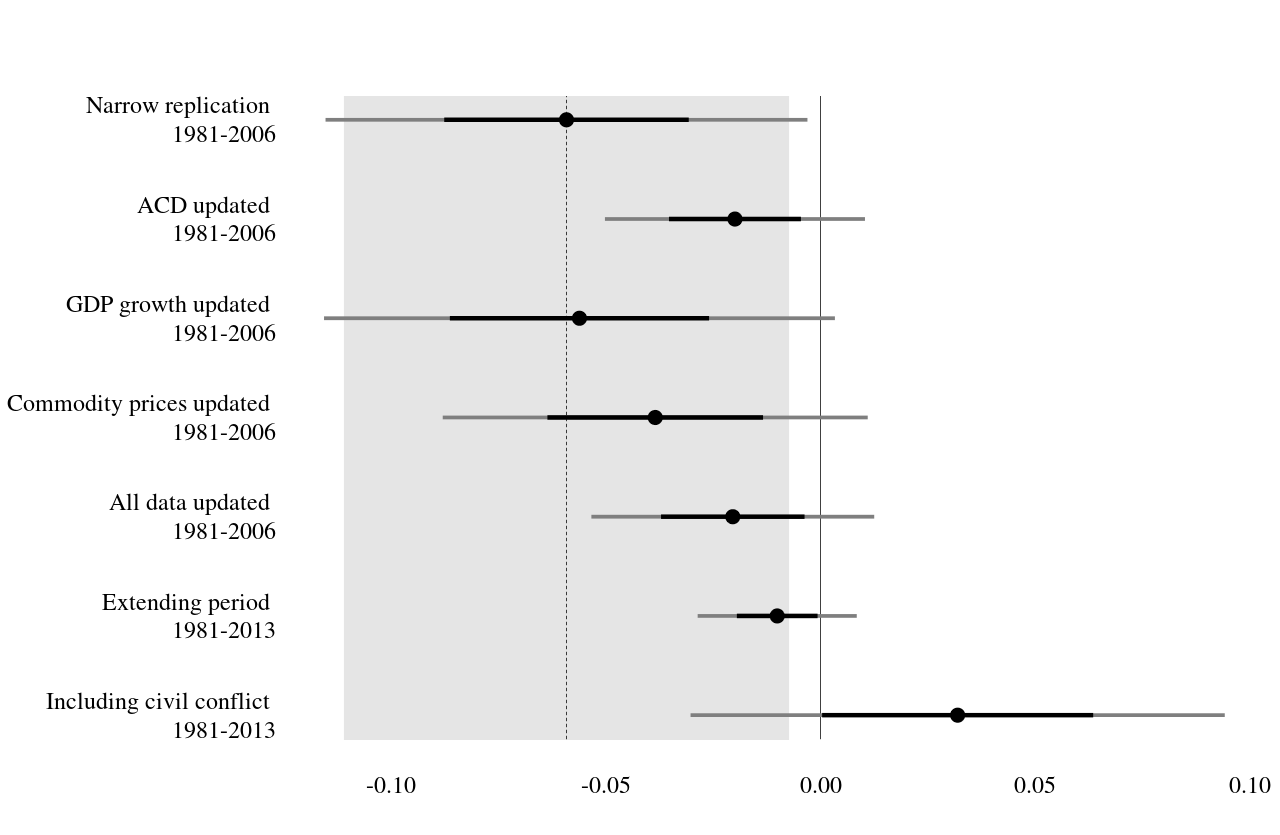
\includegraphics[width=1\textwidth]{coefplot.png}
    \caption{Coefficient estimates along with their 68\% and 95\% intervals from a reduced form model. The grey shaded area is the 95\% interval of the original estimate, with the dotted line indicating the point estimate. ACD stands for Armed Conflict Dataset.}
    \label{fig:coefplot}
\end{figure}
%**************************************
Figure~\ref{fig:coefplot} shows the estimates and their 68\% and 95\% intervals for the various replication and re-analysis attempts.  
Using the updated armed conflict data for 1981-2006, I get a much lower point estimate and the effect of commodity price shocks on civil war ceases to be statistically significant. 
This result reflects the findings by \citet{Bazzi2014} in their study on the link between commodity prices and conflict.
They comment that the relationship between commodity price shocks and conflict in the B\&C results is driven by the use of an older version of the UCDP/PRIO Armed Conflict Dataset. 
I do find that using the original coding for the outcome variable but using recent data on income or commodity prices yields similar results to the B\&C estimates although the estimated effect ceases to be statistically significant at the 5\% level.\footnote{See table~\ref{table:new_outcome},~\ref{table:new_income},~\ref{table:new_index} for results.}\\\\
% Extending the period  
Extending the period I do not find a link between commodity price shocks and civil war or civil conflict.\footnote{Civil conflict include all armed violent conflict with at least 25 battle-related deaths in a year. For civil war the threshold is 1000.}
Focussing on the extended period, turning the attention to the IV-2SLS estimation, I find in the first stage regression the commodity price index ceases to be a good instrument for GDP per capita growth.
It fails to reach statistical significance at the traditional boundaries and has a very small magnitude as shown in table~\ref{table:IV-2SLS}
Although GDP per capita is still robustly correlated with civil war onset, changes in commodity prices have very little descriptive power as the both the reduced form and second stage regression shown (column 4 and 6).
Changing the outcome variable to include the onset of all civil conflicts does not alter the conclusions.\footnote{See table~\ref{table:IV-2SLS2} for the results.}
I only found a statistically significant effect in re-estimating the model in column 1 of their table 2 changing the outcome variable to capture the outbreak of civil conflicts, these are all conflicts with at least 25 battle-related deaths in a given year. 
Contemporaneous changes in the commodity prices index were positively associated where a 20\% increase in countries' commodity price indices corresponds with a 1.6 percentage point increase in the probability of conflict onset which is statistically significant at the 5\% level (see table ~\ref{table:replication}).
In contrast with the estimation results for the model focussing solely on the effect of changes in international commodity prices, including the additional instrument (export-weighted OECD growth), does show a statistically significant link between OECD growth and civil war both in the reduced form (column 5) and in the second-stage estimation (column 7).
These results show that for a longer period of time there continues to be a negative effect of economic growth on civil war onset. 
Interestingly, this effect disappears when including civil conflict onsets in the measurement of the outcome variable (see table~\ref{table:IV-2SLS2}).\\
%**************************************
%%%% Table: IV-2SLS %%%%
%**************************************
\begin{table}[!h] \centering
  \caption{Commodity prices, export demand, and civil war onset 1981-2013}
  \label{table:IV-2SLS}
  \scalebox{0.75}{
    \begin{tabular}{@{\extracolsep{6pt}}lccccccc}
\\[-1.8ex]\hline 
\hline \\[-1.8ex]
~ &\multicolumn{2}{c}{\textit{GDP growth}}&\multicolumn{5}{c}{\textit{Civil war onset}}\\
\cmidrule(lr{1em}){2-3} \cmidrule(lr{1em}){4-8} 
\\[-1.8ex]
\textit{Specifications}       & (1)   & (2)        & (3)         & (4)       & (5)       & (6)  & (7)\\
~                             & OLS   & OLS        & OLS         & OLS       & OLS       & 2SLS & 2SLS\\
\hline \\[-1.8ex]\\	
\pbox{4cm}{3-year commodity \\ price growth} & 0.005 & 0.006      & ~           & $-$0.007  & $-$0.007  & ~    & ~\\
~                             & (1.10)& (1.30)     & ~           & ($-$0.74) & ($-$0.77) & ~    & ~\\
OECD growth                   & ~     & 0.011      & ~           & ~         & $-$0.004  & ~    & ~ \\
~                             & ~     & (12.30)*** & ~           & ~         & ($-$2.62)***& ~  & ~\\
GDP per capita growth         & ~     & ~          & $-$0.348    & ~         & ~         & $-$1.377 & $-$0.426\\
~                             & ~     & ~          & ($-$2.80)***& ~         & ~         & ($-$0.74)  & ($-$2.89)***\\
\\[-1.8ex]\\
Number of instruments         & $-$   & $-$        & $-$         & $-$       & $-$       & 1    & 2\\  
Adjusted $R^2$                & 0.117 & 0.142      & 0.131       & 0.113     & 0.113     & $-$  & $-$\\
Mean squared error            & 0.004 & 0.003      & 0.020       & 0.021     & 0.21      & 0.021& 0.021\\
\\[-1.8ex]\hline  
\hline \\[-1.8ex]
\multicolumn{8}{p{20cm}}{\textit{Notes.} All models include country and year fixed effects as well as a country-specific time trend. The first-stage estimation for column 6 is column 1 and the first-stage estimation for column 7 is column 2. $t$-values, reported in parentheses, are based on robust standard errors clustered at the country level. $N=1102$. *** p$\leq$ 0.01, ** p$\leq$ 0.05, *$\leq$ 0.1}
    \end{tabular}}
\end{table}
%**************************************
%%%% Conclusions %%%%
%**************************************
\section{Conclusions}
In this replication exercise I repeated the study by B\&C on the effect of changes in international commodity prices on the probability of conflict onset. 
Using R to estimate the model I find that I am able to replicate their results although there are some discrepancies, caused by a small sample adjustment used in the calculation of the standard errors.
The original results are not robust to coding the outcome variable using the most recent data on armed conflict. 
Extending the period, I am unable to establish a strong relation between commodity prices and civil war for 1981-2013. 
However, estimating the model with instrumenting economic growth with both international commodity prices and economic growth in OECD export countries I find that for the period 1981-2013 economic growth negatively affects civil war onset. 
%**************************************
%%%% References %%%%
%**************************************
\let\oldbibliography\thebibliography
\renewcommand{\thebibliography}[1]{\oldbibliography{#1}
\setlength{\itemsep}{0pt}} %Reducing spacing in the bibliography.
\def\bibfont{\footnotesize}
\bibliographystyle{chicago}
\bibliography{rep}
\newpage
%**************************************
%%%% Appendix %%%%
%**************************************
\appendix
\section{Supporting information}
\subsection{Tables replication results}
\setcounter{table}{0}
\renewcommand{\thetable}{A\arabic{table}}
\setcounter{figure}{0}
\renewcommand{\thefigure}{A\arabic{figure}}
%**************************************
%%%% Table 2 %%%%
%**************************************
\begin{table}[!h] \centering
  \caption{Commodity price shocks and civil war onset 1981-2006}
  \label{table:2}
  \scalebox{0.75}{
    \begin{tabular}{@{\extracolsep{6pt}}lccccccc}
\\[-1.8ex]\hline 
\hline \\[-1.8ex]
~ &\multicolumn{6}{c}{\textit{Civil war onset}}\\
\cmidrule(lr{1em}){2-7} 
\\[-1.8ex]
\textit{Specifications}       & (1)         & (2)       & (3)          & (4)        & (5)     & (6)\\
\hline \\[-1.8ex]\\	
Commodity price growth, $t$   & $-$0.055    & ~         & $-$0.054     & $-$0.051   & ~       & ~\\
~                             & ($-$1.76)*  & ~         & ($-$1.72)*   & ($-$1.66)* & ~       & ~\\
Commodity price growth, $t-1$ & $-$0.028    & ~         & $-$0.029     & $-$0.027   & ~       & ~\\
~                             & ($-$0.73)   & ~         & ($-$0.75)    & ($-$0.69)  & ~       & ~\\
Commodity price growth, $t-2$ & $-$0.087    & ~         & $-$0.087     & $-$0.084   & ~       & ~\\
~                             & ($-$2.05)** & ~         & ($-$2.03)**  & ($-$1.96)**& ~       & ~\\
\\[-1.8ex]\\
3-year commodity price growth & ~           & ~         & ~            & ~          & $-$0.059  & $-$0.058\\
~                             & ~           & ~         & ~            & ~          & ($-$2.07)** & ($-$2.03)**\\
\\[-1.8ex]\\
Rainfall growth, $t$          & ~           & $-$0.007  & $-$0.006     & ~          & ~       & ~\\
~                             & ~           & ($-$0.29) & ($-$0.25)    & ~          & ~       & ~\\
Rainfall growth, $t-1$        & ~           & $-$0.005  & $-$0.005     & ~          & ~       & ~\\
~                             & ~           & ($-$0.19) & ($-$0.19)    & ~          & ~       & ~\\
Rainfall growth, $t-2$        & ~           & $-$0.18   & $-$0.015     & ~          & ~       & ~\\
~                             & ~           & ($-$0.52) & ($-$0.43)    & ~          & ~       & ~\\
\\[-1.8ex]\\
Log rainfall, $t$             & ~           & ~         & ~            & $-$0.031   & ~       & ~\\
~                             & ~           & ~         & ~            & ($-$0.85)  & ~       & ~\\
Log rainfall, $t-1$           & ~           & ~         & ~            & $-$0.047   & ~       & ~\\
~                             & ~           & ~         & ~            & ($-$1.47)  & ~       & ~\\
Log rainfall, $t-2$           & ~           & ~         & ~            & $-$0.007   & ~       & ~\\
~                             & ~           & ~         & ~            & ($-$0.14)  & ~       & ~\\
\\[-1.8ex]\\            
3-year rainfall               & ~           & ~         & ~            & ~          & ~       & $-$0.091\\
~                             & ~           & ~         & ~            & ~          & ~       &($-$1.41)\\
\\[-1.8ex]\\      
Adjusted $R^2$                & 0.166       & 0.157     & 0.162        & 0.165      & 0.168   & 0.169\\
Mean squared error            & 0.020       & 0.020     & 0.020        & 0.020      & 0.020   & 0.20\\
\\[-1.8ex]\hline 
\hline \\[-1.8ex]
\multicolumn{7}{p{20cm}}{\textit{Notes.} Models are estimated using OLS and all models include country and year fixed effects as well as a country-specific time trend. $t$-values, reported in parentheses, are based on robust standard errors clustered at the country level. $N=814$. *** p$\leq$ 0.01, ** p$\leq$ 0.05, *$\leq$ 0.1}
    \end{tabular}}
\end{table}
%**************************************
%%%% Table 3 %%%%
%**************************************
\begin{table}[!h] \centering
  \caption{Limited dependent variable estimates}
  \label{table:3}
  \scalebox{0.75}{
    \begin{tabular}{@{\extracolsep{6pt}}lcccccccc}
\\[-1.8ex]\hline 
\hline \\[-1.8ex]
~ &\multicolumn{6}{c}{\textit{Civil war onset}}\\
\cmidrule(lr{1em}){2-8} 
\\[-1.8ex]
~                        & (1)         & (2)       & (3)          & (4)        & (5)     & (6) & (7)\\
\\[-1.8ex]
~&\multicolumn{3}{c}{Marginal effects} &~ &~ &~ &~\\
\cmidrule(lr{1em}){2-4} 
\\[-1.8ex]
~                         &OLS          &Probit     &Logit         &Logit       &Rare event Logit& Logit& Logit\\
\hline \\[-1.8ex]\\	
\pbox{5cm}{3-year commodity \\ price growth}
 & $-$0.027  & $-$0.034  & $-$0.034  & $-$1.351  & $-$1.248 & $-$1.467 & $-$8.081\\
~                             & ($-$1.80)*& ($-$1.75)*& ($-$1.65)*& ($-$1.65)*& ($-$1.53)& ($-$2.35)** & ($-$2.56)**\\
\\[-1.8ex]\\  
Country FE                    & $-$       & $-$       & $-$       & $-$       & $-$      & Yes  & Yes\\
Time Trends                   & $-$       & $-$       & $-$       & $-$       & $-$      & $-$  & Yes\\
Year FE                       & $-$       & $-$       & $-$       & $-$       & $-$      & $-$  & Yes\\
\\[-1.8ex]\hline 
\hline \\[-1.8ex]
\multicolumn{8}{p{15cm}}{\textit{Notes.} $N=814$. $t$ or $z$-values, reported in parentheses, are based on robust standard errors clustered at the country level. *** p$\leq$ 0.01, ** p$\leq$ 0.05, *$\leq$ 0.1}
    \end{tabular}}
\end{table}
%**************************************
%%%% Table 4 %%%%
%**************************************
\begin{table}[!h] \centering
  \caption{Economic growth and civil war onset 1981-2006}
  \label{table:4}
  \scalebox{0.75}{
    \begin{tabular}{@{\extracolsep{6pt}}lccc}
\\[-1.8ex]\hline 
\hline \\[-1.8ex]
~ &\multicolumn{1}{c}{\textit{GDP growth}}&\multicolumn{2}{c}{\textit{Civil war onset}}\\
\cmidrule(lr{1em}){2-2} \cmidrule(lr{1em}){3-4} 
\\[-1.8ex]
\textit{Specifications}       & (1)         & (2)         & (3)\\
~                             & OLS         & OLS         & 2SLS\\        
\hline \\[-1.8ex]\\	
3-year commodity price growth & 0.028       & ~           & ~\\
~                             & (3.67)***   & ~           & ~\\
GDP per capita growth         & ~           & $-$0.367    & $-$2.091\\
~                             & ~           & ($-$2.38)** & ($-$2.07)**\\
\\[-1.8ex]\\  
Adjusted $R^2$                & 0.041       & 0.194       & ~\\
Mean squared error            & 0.006       & 0.019       & 0.020\\
\\[-1.8ex]\hline  
\hline \\[-1.8ex]
\multicolumn{4}{p{10cm}}{\textit{Notes.} All models include country and year fixed effects as well as a country-specific time trend. $t$-values, reported in parentheses, are based on robust standard errors clustered at the country level. $N=814$. *** p$\leq$ 0.01, ** p$\leq$ 0.05, *$\leq$ 0.1}
    \end{tabular}}
\end{table}
%**************************************
%%%% Table 5 %%%%
%**************************************
\begin{table}[!h] \centering
  \caption{Export demand, economic growth, and civil war onset 1981-2006}
  \label{table:5}
  \scalebox{0.75}{
    \begin{tabular}{@{\extracolsep{6pt}}lccc}
\\[-1.8ex]\hline 
\hline \\[-1.8ex]
~ &\multicolumn{1}{c}{\textit{GDP growth}}&\multicolumn{2}{c}{\textit{Civil war onset}}\\
\cmidrule(lr{1em}){2-2} \cmidrule(lr{1em}){3-4} 
\\[-1.8ex]
\textit{Specifications}       & (1)         & (2)         & (3)\\
~                             & OLS         & OLS         & 2SLS\\        
\hline \\[-1.8ex]\\	
3-year commodity price growth & 0.031       & $-$0.061    & ~\\
~                             & (3.64)***   & ($-$2.13)** & ~\\
OECD growth                   & 0.010       & $-$0.006    & ~\\
~                             & (16.28)***  & ($-$5.40)***& ~\\
GDP per capita growth         & ~           & ~           & $-$0.813\\
~                             & ~           & ~           & ($-$6.00)***\\
\\[-1.8ex]\\  
Adjusted $R^2$                & 0.103       & 0.174       & ~\\
Mean squared error            & 0.006       & 0.020       & 0.020\\
\\[-1.8ex]\hline  
\hline \\[-1.8ex]
\multicolumn{4}{p{10cm}}{\textit{Notes.} All models include country and year fixed effects as well as a country-specific time trend. $t$-values, reported in parentheses, are based on robust standard errors clustered at the country level. $N=814$. *** p$\leq$ 0.01, ** p$\leq$ 0.05, *$\leq$ 0.1}
    \end{tabular}}
\end{table}
%**************************************
%%%% Table 6 %%%%
%**************************************
\begin{table}[!h] \centering
  \caption{Economic growth and civil conflict onset 1981-2006}
  \label{table:6}
  \scalebox{0.75}{
    \begin{tabular}{@{\extracolsep{6pt}}lcccc}
\\[-1.8ex]\hline 
\hline \\[-1.8ex]
~ &\multicolumn{1}{c}{\textit{GDP growth}}&\multicolumn{3}{c}{\textit{Civil war onset}}\\
\cmidrule(lr{1em}){2-2} \cmidrule(lr{1em}){3-5} 
\\[-1.8ex]
\textit{Specifications}       & (1)         & (2)         & (3)     & (4)\\
~                             & OLS         & OLS         & OLS     & 2SLS\\        
\hline \\[-1.8ex]\\	
3-year commodity price growth & 0.025       & $-$0.033    & ~       & ~\\
~                             & (2.28)**    & ($-$0.91)   & ~       & ~\\
OECD growth                   & 0.010       & $-$0.005    & ~       & ~\\
~                             & (13.99)***  & ($-$3.19)***& ~       & ~\\
GDP per capita growth         & ~           & ~           & $-$0.310&$-$0.619\\
~                             & ~           & ~           & ($-$2.04)**&($-$2.78)***\\
\\[-1.8ex]\\  
Adjusted $R^2$                & 0.152       & 0.166       & 0.175   &~\\
Mean squared error            & 0.005       & 0.037       & 0.037   & 0.037\\
\\[-1.8ex]\hline  
\hline \\[-1.8ex]
\multicolumn{4}{p{10cm}}{\textit{Notes.} All models include country and year fixed effects as well as a country-specific time trend. $t$-values, reported in parentheses, are based on robust standard errors clustered at the country level. $N=688$. *** p$\leq$ 0.01, ** p$\leq$ 0.05, *$\leq$ 0.1}
    \end{tabular}}
\end{table}
\clearpage
%**************************************
%%%% Reanalysis tables and figures %%%%
%**************************************
\subsection{Tables and figures reanalysis results}
\setcounter{table}{0}
\renewcommand{\thetable}{B\arabic{table}}
\setcounter{figure}{0}
\renewcommand{\thefigure}{B\arabic{figure}}
%**************************************
%%%% Figure: Conflict trends %%%%
%**************************************
\begin{figure}[!h]
\centering
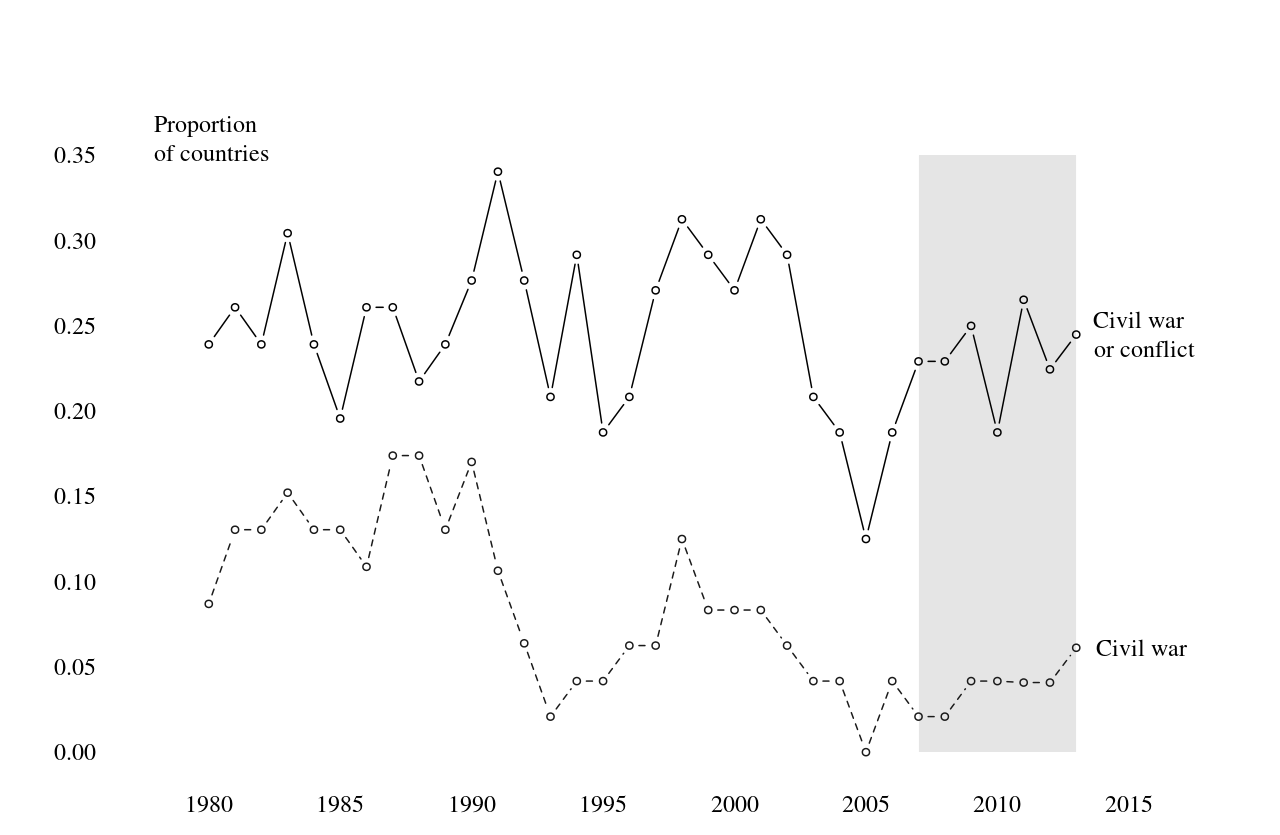
\includegraphics[width=1\textwidth]{proportion.png}\\ 
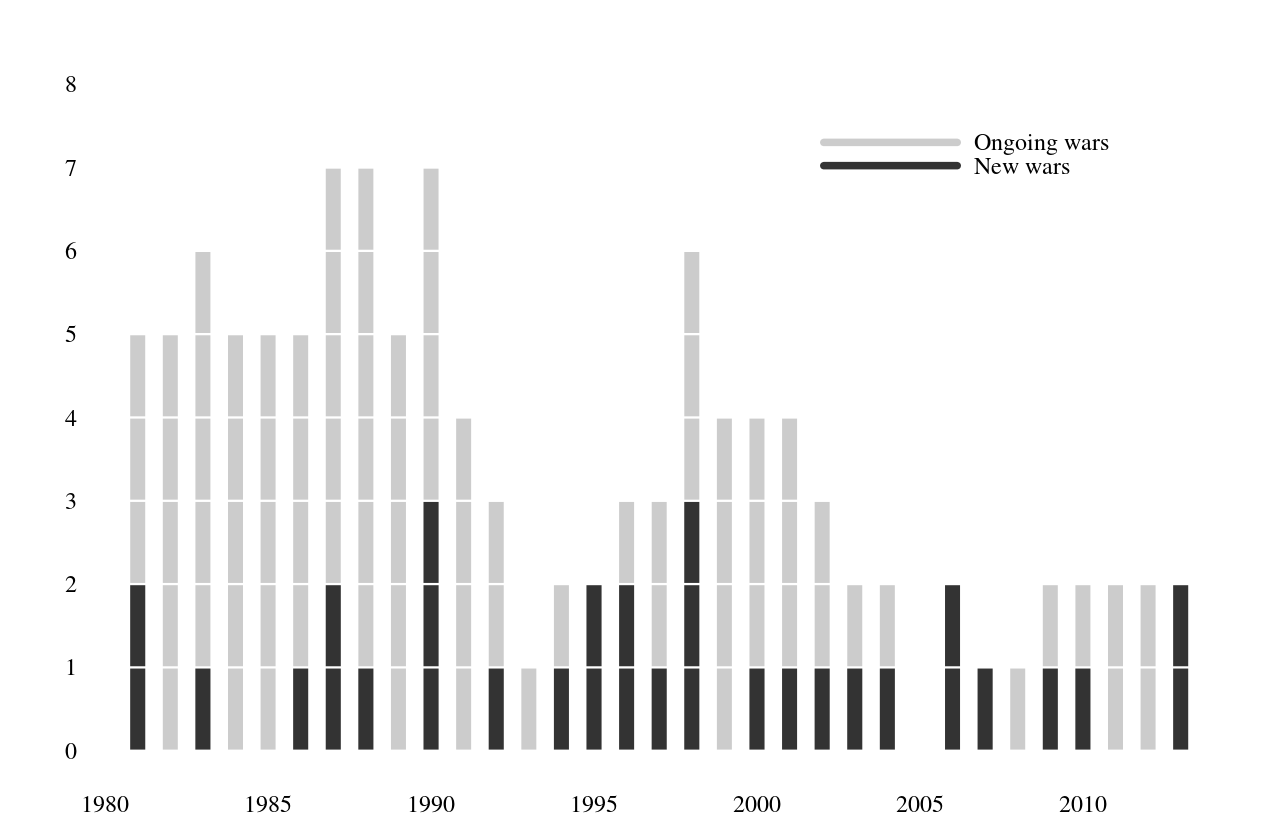
\includegraphics[width=1\textwidth]{ongoing_onset.png}
\caption[Conflict trends over time]{\textbf{Top:} Proportion of Sub-Sahara African countries with active civil conflict/war, 1980-2013. The grey area indicates the extended period for the re-analysis 2007-2013. \textbf{Bottom:} Incidence and onset of civil war in Sub-Sahara Africa, 1980-2013. $Source:$ UCDP/PRIO.}
\label{fig:conflict_trends}
\end{figure}
%**************************************
%%%% Table: Descriptive statistics %%%%
%**************************************
\begin{table}[!h] \centering \normalsize
  \caption{Descriptive statistics 1981-2013}
  \label{table:ds}
\scalebox{0.75}{\begin{tabular}{@{\extracolsep{5pt}}lcccccc}
\\[-1.8ex]\hline 
\hline \\[-1.8ex] 
Variable                       & $N$ & Mean & \pbox{4cm}{Standard \\ deviation}  & Min. & Median & Max.\\[-1.8ex]\\
\hline \\[-1.8ex]\\
    Civil war onset                        & 1196 & 0.03  & 0.16  & 0 & 0 & 1\\
    Civil conflict onset                   & 1034 & 0.06  & 0.24  & 0 & 0 & 1\\
   \\[-1.8ex] \\
    3-year commodity price index growth    & 1202 & 0.14  & 0.48  & $-$0.68 & 0.03  & 5.60\\
    Commodity price index growth$_{t}$     & 1278 & 0.04  & 0.23  & $-$0.62 & 0.002 & 3.23\\
    OECD GDP growth index$_{t}$            & 1278 & 0.01  & 0.02  & $-$0.14 & 0.002 & 0.22\\
    GDP per capita growth$_{t}$            & 1233 & 0.01  & 0.07  & $-$0.50 & 0.01  & 0.92\\
    \\[-1.8ex] \\
\hline \\[-1.8ex]
    \end{tabular}}
\end{table} 
%**************************************
%%%% Table: Data changes conflict %%%%
%**************************************
\begin{table}[!h] \centering \caption{Civil war onset years per country} \label{table:war}
\scalebox{0.75}{\begin{tabular}{lll}
\\[-1.8ex]\hline 
\hline \\[-1.8ex] 
Country & B\&C data (1981-2006) & Re-analysis data (1981-2013)\\
\hline \\[-1.8ex]\\
Angola          & \textbf{1998}
                & 1992, \textbf{1998}\\ 
Burundi         & 1998, \textbf{2000}
                & \textbf{2000}\\
Chad            & \textbf{1990}, \textbf{2006} 
                & 1987, \textbf{1990}, \textbf{2006}\\ 
DRC             & 1997      
                & 1996, 2013*\\
Congo           & \textbf{1997}
                & \textbf{1997}\\
Ethiopia        & $-$
                & 1987\\                
Guinea-Bissau   & 1998  
                & $-$\\
Liberia         & 1990, 1992, \textbf{2003} 
                & \textbf{2003}\\
Mozambique      & \textbf{1981} 
                & \textbf{1981}\\
Nigeria         & $-$
                & 2013*\\
Rwanda          & 1991, \textbf{1998}, \textbf{2001} 
                & 1990, 1994, \textbf{1998}, \textbf{2001},2009*\\
Sierra Leone    & \textbf{1998}  
                & 1995, \textbf{1998}\\
Somalia         & 1989      
                & 1988, 1990, 2007*\\
South Africa    & \textbf{1986}  
                & \textbf{1986}\\
Sudan           & \textbf{1983}, \textbf{1995}, \textbf{2006} 
                & \textbf{1983}, \textbf{1995}, \textbf{2006}, 2010*\\
Uganda          & \textbf{1981}, 1991, \textbf{2002}, \textbf{2004} 
                & \textbf{1981}, 1996, \textbf{2002}, \textbf{2004}\\
    \\[-1.8ex]\hline 
    \hline \\[-1.8ex]
\multicolumn{3}{p{12cm}}{\textit{Notes.} DRC stands for the Democratic Republic of the Congo. BC data refers to the dataset used by \citet{Bruckner2010}. The re-analysis data on the outcome variable is taken from UCDP/PRIO Armed Conflict Dataset v.4-2014a, 1946 – 2013. Years denoted with an asterisk indicate years that were not included in the BC sample (2007-2013). The years printed in bold typeface indicate civil war onset years that are identical across the two datasets. The changes between the two datasets seems to be largely driven by the changes made in the practice of coding startdates as mentioned in the \href{http://www.pcr.uu.se/digitalAssets/124/124920_1version_history_v4-2014a.pdf}{version history} of the armed conflict dataset.}
\end{tabular} }  
\end{table}
%**************************************
%%%% Table: Replication conflict onset %%%%
%**************************************
\begin{table}[!h] \centering
  \caption{Commodity price shocks and conflict onset}
  \label{table:replication}
  \scalebox{0.7}{
    \begin{tabular}{@{\extracolsep{6pt}}lcccccc}
\\[-1.8ex]\hline 
\hline \\[-1.8ex]
~ &\multicolumn{4}{c}{\textit{Civil war onset}} &\multicolumn{2}{c}{\textit{Civil conflict onset}}\\
\cmidrule(lr{1em}){2-5} \cmidrule(lr{1em}){6-7}
\\[-1.8ex]
~&\multicolumn{2}{c}{1981-2006} &\multicolumn{4}{c}{1981-2013}\\
\cmidrule(lr{1em}){2-3} \cmidrule(lr{1em}){4-7}
\textit{Specifications}       & (1)         & (2)       & (3)        & (4)      & (5)     & (6)\\
\hline \\[-1.8ex]\\	
Commodity price growth, $t$   & $-$0.018    & ~         & $-$0.008   & ~        & 0.081   & ~\\
~                             & ($-$0.43)   & ~         & ($-$0.32)  & ~        & (1.99)**& ~\\
Commodity price growth, $t-1$ & $-$0.024    & ~         & $-$-0.012  & ~        &$-$0.028 & ~\\
~                             & ($-$0.75)   & ~         & ($-$0.53)  & ~        & ($-$0.52)& ~\\
Commodity price growth, $t-2$ & $-$0.008    & ~         & $-$0.013   & ~        & 0.027   & ~\\
~                             & ($-$0.15)   & ~         & ($-$0.50)  & ~        & (0.65)  & ~\\
\\[-1.8ex]\\
3-year commodity price growth & ~           & $-$0.020  & ~          & $-$0.010 & ~       & 0.032\\
~                             & ~           & ($-$1.22) & ~          & ($-$1.07)&~        & (1.01)\\
\\[-1.8ex]\\
Adjusted $R^2$                & 0.095       & 0.010     & 0.078      & 0.080    & 0.120   & 0.120\\
Mean squared error            & 0.022       & 0.022     & 0.022      & 0.022    & 0.045   & 0.046\\
$N$                           & 862         & 862       & 1128       & 1128     & 970     & 970\\
\\[-1.8ex]\hline 
\hline \\[-1.8ex]
\multicolumn{7}{p{15cm}}{\textit{Notes.} Models are estimated using OLS and all models include country and year fixed effects as well as a country-specific time trend. $t$-values, reported in parentheses, are based on robust standard errors clustered at the country level. *** p$\leq$ 0.01, ** p$\leq$ 0.05, *$\leq$ 0.1}
    \end{tabular}}
\end{table}
%**************************************
%%%% Table: IV-2SLS %%%%
%**************************************
\begin{table}[!h] \centering
  \caption{Commodity prices, export demand, and civil conflict onset 1981-2013}
  \label{table:IV-2SLS2}
  \scalebox{0.75}{
    \begin{tabular}{@{\extracolsep{6pt}}lccccccc}
\\[-1.8ex]\hline 
\hline \\[-1.8ex]
~ &\multicolumn{2}{c}{\textit{GDP growth}}&\multicolumn{5}{c}{\textit{Civil conflict onset}}\\
\cmidrule(lr{1em}){2-3} \cmidrule(lr{1em}){4-8} 
\\[-1.8ex]
\textit{Specifications}       & (1)   & (2)        & (3)         & (4)       & (5)       & (6)  & (7)\\
~                             & OLS   & OLS        & OLS         & OLS       & OLS       & 2SLS & 2SLS\\
\hline \\[-1.8ex]\\	
3-year commodity price growth & 0.009 & 0.010      & ~           & 0.036     & 0.036     & ~    & ~\\
~                             & (1.57)& (1.70)*    & ~           & (1.12)    & (1.12)    & ~    & ~\\
OECD growth                   & ~     & 0.009      & ~           & ~         & 0.001     & ~    & ~ \\
~                             & ~     & (9.81)***  & ~           & ~         & (0.59)    & ~    & ~\\
GDP per capita growth         & ~     & ~          & $-$0.19     & ~         & ~         & 3.836&0.562\\
~                             & ~     & ~          & ($-$1.16)   & ~         & ~         & (1.12)  &(0.85)\\
\\[-1.8ex]\\
Number of instruments         & $-$   & $-$        & $-$         & $-$       & $-$       & 1    & 2\\  
Adjusted $R^2$                & 0.139 & 0.163      & 0.131       & 0.132     & 0.131     & $-$  & $-$\\
Mean squared error            & 0.003 & 0.003      & 0.044       & 0.044     & 0.044     & 0.044& 0.044\\
\\[-1.8ex]\hline  
\hline \\[-1.8ex]
\multicolumn{8}{p{15cm}}{\textit{Notes.} All models include country and year fixed effects as well as a country-specific time trend. The first-stage estimation for column 6 is column 1 and the first-stage estimation for column 7 is column 2. $t$-values, reported in parentheses, are based on robust standard errors clustered at the country level. $N=951$. *** p$\leq$ 0.01, ** p$\leq$ 0.05, *$\leq$ 0.1}
    \end{tabular}}
\end{table}
%**************************************
%%%% Table IV-2SLS: Civil war %%%%
% New data outcome variable
%**************************************
\begin{table}[!h] \centering
  \caption{Economic growth and civil war onset 1981-2006 \\ \textit{New data onset variable }}
  \label{table:new_outcome}
  \scalebox{0.75}{
    \begin{tabular}{@{\extracolsep{6pt}}lcccc}
\\[-1.8ex]\hline 
\hline \\[-1.8ex]
~ &\multicolumn{1}{c}{\textit{GDP growth}}&\multicolumn{3}{c}{\textit{Civil war onset}}\\
\cmidrule(lr{1em}){2-2} \cmidrule(lr{1em}){3-5} 
\\[-1.8ex]
\textit{Specifications}       & (1)         & (2)         & (3)       & (4)\\
~                             & OLS         & OLS         & OLS       & 2SLS\\        
\hline \\[-1.8ex]\\	
3-year commodity price growth & 0.025       & ~           & $-$0.020  & ~\\
~                             & (3.19)**    & ~           & ($-$1.29) & ~\\
GDP per capita growth         & ~           & $-$0.186    & ~         & $-$0.792\\
~                             & ~           & ($-$2.04)** & ~         & ($-$1.29)\\
\\[-1.8ex]\\  
Adjusted $R^2$                & 0.033       & 0.119       & 0.110     & $-$\\
Mean squared error            & 0.007       & 0.022       & 0.022     & 0.022\\
\\[-1.8ex]\hline  
\hline \\[-1.8ex]
\multicolumn{5}{p{15cm}}{\textit{Notes.} All models include country and year fixed effects as well as a country-specific time trend. $t$-values, reported in parentheses, are based on robust standard errors clustered at the country level. $N=829$. *** p$\leq$ 0.01, ** p$\leq$ 0.05, *$\leq$ 0.1}
    \end{tabular}}
\end{table}
%**************************************
%%%% Table: IV-2SLS: Civil war %%%%
% New data income
%**************************************
\begin{table}[!h] \centering
  \caption{Economic growth and civil war onset 1981-2006 \\ \textit{New data GDP variable }}
  \label{table:new_income}
  \scalebox{0.75}{
    \begin{tabular}{@{\extracolsep{6pt}}lcccc}
\\[-1.8ex]\hline 
\hline \\[-1.8ex]
~ &\multicolumn{1}{c}{\textit{GDP growth}}&\multicolumn{3}{c}{\textit{Civil war onset}}\\
\cmidrule(lr{1em}){2-2} \cmidrule(lr{1em}){3-5} 
\\[-1.8ex]
\textit{Specifications}       & (1)         & (2)         & (3)       & (4)\\
~                             & OLS         & OLS         & OLS       & 2SLS\\        
\hline \\[-1.8ex]\\	
3-year commodity price growth & 0.016       & ~           & $-$0.056  & ~\\
~                             & (2.56)**    & ~           & ($-$1.85)*& ~\\
GDP per capita growth         & ~           & $-$0.540    & ~         & $-$3.509\\
~                             & ~           & ($-$2.74)***& ~         & ($-$1.85)*\\
\\[-1.8ex]\\  
Adjusted $R^2$                & 0.090       & 0.235       & 0.195     & $-$\\
Mean squared error            & 0.004       & 0.018       & 0.019     & 0.019\\
\\[-1.8ex]\hline  
\hline \\[-1.8ex]
\multicolumn{5}{p{15cm}}{\textit{Notes.} All models include country and year fixed effects as well as a country-specific time trend. $t$-values, reported in parentheses, are based on robust standard errors clustered at the country level. $N=773$. *** p$\leq$ 0.01, ** p$\leq$ 0.05, *$\leq$ 0.1}
    \end{tabular}}
\end{table}
%**************************************
%%%% Table: IV-2SLS: Civil war %%%%
% New data index
%**************************************
\begin{table}[!h] \centering
  \caption{Economic growth and civil war onset 1981-2006 \\ \textit{New data price variable }}
  \label{table:new_index}
  \scalebox{0.75}{
    \begin{tabular}{@{\extracolsep{6pt}}lcccc}
\\[-1.8ex]\hline 
\hline \\[-1.8ex]
~ &\multicolumn{1}{c}{\textit{GDP growth}}&\multicolumn{3}{c}{\textit{Civil war onset}}\\
\cmidrule(lr{1em}){2-2} \cmidrule(lr{1em}){3-5} 
\\[-1.8ex]
\textit{Specifications}       & (1)         & (2)         & (3)       & (4)\\
~                             & OLS         & OLS         & OLS       & 2SLS\\        
\hline \\[-1.8ex]\\	
3-year commodity price growth & 0.025       & ~           & $-$0.038  & ~\\
~                             & (2.92)***   & ~           & ($-$1.52) & ~\\
GDP per capita growth         & ~           & $-$0.540    & ~         & $-$1.564\\
~                             & ~           & ($-$2.74)***& ~         & ($-$1.52)\\
\\[-1.8ex]\\  
Adjusted $R^2$                & 0.037       & 0.235       & 0.175     & $-$\\
Mean squared error            & 0.006       & 0.018       & 0.019     & 0.019\\
\\[-1.8ex]\hline  
\hline \\[-1.8ex]
\multicolumn{5}{p{15cm}}{\textit{Notes.} All models include country and year fixed effects as well as a country-specific time trend. $t$-values, reported in parentheses, are based on robust standard errors clustered at the country level. $N=796$. *** p$\leq$ 0.01, ** p$\leq$ 0.05, *$\leq$ 0.1}
    \end{tabular}}
\end{table}
\end{document}
